\documentclass[../Main/Main.tex]{subfiles}

\begin{document}
Pasar de un modelo tan estructurado a su implementación computacional no resulto fácil. Sin embargo, se logró desarrollar un algoritmo que estima todos los parámetros del modelo de una forma eficiente y que funciona en la práctica. En el fondo, el algoritmo recae en el método de Gibbs sampling propuesto en \autocite{albert1993bayesian}, por lo que se hace una breve introducción a la escuela de inferencia bayesiana, y en el algortimo de backfitting descrito en \autocite{hastie1986generalized}. Al algoritmo se le titula: \textit{bayesian piece wise polinomial model (bpwpm)}. Para facilitar la utilización del modelo en diversas bases de datos, así como  su validación y visualización, a la par del algoritmo se desarrolló un paquete de código abierto (con el mismo nombre) para el software estadístico \verb|R|. Al darle un tratamiento bayesiano a los parámetros, más que estimarlos, se busca regresar una muestra de tamaño arbitrario de sus correspondientes distribuciones posteriores. La idea, es que estas distribuciones posteriores, se haya capturado toda la información de los datos de entrenamiento. \\

Se considera, que una buena forma de entender el algoritmo es \textit{visualizando} tanto los datos como los objetos que componen el modelo, por lo tanto se hace un paréntesis notacional. De las ecuaciones del modelo: (\ref{ec:Y-Z}) a (\ref{ec:fj}), se tienen dos grupos de parámetros por estimar, $\beta \in \mathbb{R}^{d+1}$ y $w_j \in \mathbb{R}^{\N} \quad \forall j = 1,\ldots,d$. Donde:
\begin{align*}
\beta &= 
\left[ 
	\begin{array}{c}
	\beta_0 \\
	\beta_1 \\ 
	\vdots \\
	\beta_d
	\end{array}\right]
\quad \text{y} \quad 
w_1 = 
\left[ 
	\begin{array}{c}
	w_{1,1}\\
	\vdots\\
	w_{1,\N}
	\end{array}\right]
\quad \ldots \quad 
w_d = 
\left[ 
	\begin{array}{c}
	w_{d,1}\\
	\vdots\\
	w_{d,\N}
	\end{array}\right]
\end{align*}
Se hace énfasis en que existen $d$ vectores $w_j$, cada uno de tamaño $\N$. Por lo tanto, se tienen sun total de $1 + d + d\N$ parámetros. Se usa el símbolo $\wsn$ para designar todos los vectores $w_j$, haciendo de este una matriz, es decir: $\wsn\in\mathbb{R}^{d\times\N}$. Cuando se habla de datos: $\{(y_i,\xni)\}_{i = 1}^n$, estos se pueden  representar en una tabla (o matriz):
$$\left[\begin{array}{c|ccc} 
y_1 & x_{1,1} & \ldots & x_{1,d} \\ 
\vdots & \vdots & ~ & \vdots \\ 
y_n & x_{n,d} & \ldots & x_{n,d}
\end{array}\right]$$
Donde el vector de observaciones binarias $\ysn = (y_1,\ldots,y_n)^t$ es la primer columna de la tabla, y la matriz de covariables $\mathbf{X}$ es el resto.\\

Bajo esta representación, se da contexto cuando se habla de que la estimación debe reflejar los patrones \textit{hacia abajo} y \textit{hacia lo largo}. Hacia abajo, se está captando la información existente entre las observaciones;  cada $f_j$, mediante su parámetro $w_j$, representa una transformación no lineal de la variable (o dimensión) $j$. Hacia lo largo, la función de proyección $f$ suma cada $f_j$ a través de $\beta$, ponderando los efectos individuales de cada variable. Mantener el balance entre la estimación de $\beta$ a lo largo y $w_j$ hacia abajo, es fundamental para el algoritmo. Analizando este hecho, se concluye que la estimación de ambos grupos de parámetros, se puede ver como una regresión separada para cada uno, y por ende, estos pueden ser estimados por el mismo algoritmo. Esto responde a la dualidad que se exploró en el capítulo pasado de que ambas expresiones son expansiones en bases funcionales. El puente que conecta, y controla el balance entre ambas, son los residuales parciales. Los siguientes capítulos, se concentran en explicar e implementar este curioso patrón. 

\section{Fundamentos de la estadística bayesiana}
Dado el problema de describir fenómenos bajo incertidumbre, existen dos escuelas dominantes de la estadística: la frecuentista y la bayesiana. La primera, aunque increíblemente útil, está hasta cierto punto limitada y en ocasiones termina derivando en colecciones de algoritmos. La teoría bayesiana, por el contrario, nombrada así en honor a Thomas Bayes (1702 - 1761), es una rama que enfatiza el componente \textit{probabilista}, dando coherencia al proceso de inferencia \autocite{mendoza2011estadistica} y \autocite{bernardo2001bayesian}. La estadistica bayesiana está  axiomatizada bajo la \textit{teoría de la decisión}. Esta teoría formaliza conceptos económicos como la \textit{coherencia entre preferencias} y \textit{utilidad}, sobre los que desarrolla un marco metodológico para la toma de decisiones. \\\

Esta metodología, además de proveer técnicas concretas para resolver problemas, también formaliza en una forma de pensar sobre la probabilidad como una \textit{medida racional para cuantificar la incertidumbre} condicionando sobre el conocimiento existente. Este paradigma es el que más corresponde con el sentido que usualmente se le da a la palabra. La inferencia sobre creencias (o parámetros), se realiza mediante una \textit{actualización} de estas en luz de nueva evidencia, modificando su medida de incertidumbre. El mecanismo que permite realizar esto, es la aclamada formula de Bayes. De manera informal se puede describir como: dado un evento $E$ bajo condiciones $C$, la probabilidad \textit{posterior} del evento, es proporcional a la probabilidad \textit{previa} que se tiene sobre este, ponderado por la probabilidad de ocurrencia de las condiciones presentes, es decir: 
\begin{align}
P(E|C) \; \alpha \; P(C|E)P(E) \label{ec:BayesInformal}
\end{align}
El término central $P(C|E)$ es una medida descriptiva de las condiciones (usualmente datos) llamada \textit{verosimilitud}. Se hace notar que para poder hacer cualquier intento de descripción, se debe especificar el \textit{modelo probablistico} que se asume describe el estado por el que se dan las condiciones $C$. \

En un contexto matemático más formal, la cuantificación de la incertidumbre se da a través de medidas de probabilidad $\pi(\cdot)$, que describan el fenómeno observado. Estas medidas de probabilidad, usualmente son funciones que dependen de cantidades desconocidas llamados parámetros $\theta$. Aunque desconocidas, se tienen ciertas creencias u conocimiento previo, \textit{a priori}, sobre ellos, descritos por su correspondiente medida de probabilidad $\pi(\theta)$. Además, se tienen datos $\mathbf{X}$, interpretados como \textit{evidencia}, a los cuales se les asigna un modelo de probabilidad dependiente de los parámetros, es decir, su verosimilitud: $\pi(\mathbf{X}|\theta)$. Usando la formula de Bayes, podemos actualizar el conocimiento que se tiene sobre los parámetros haciendo:
\begin{align}
	\pi(\theta|\mathbf{X}) \; \alpha \; \pi(\mathbf{X}|\theta)\pi(\theta) \label{ec:BayesProporcional}
\end{align}
La idea es que este proceso de actualización sea a la vez, un proceso de aprendizaje, en el cual los parámetros capturen la información contenida en los datos.\\

La teoría frecuentista, adopta un enfoque diferente para el  aprendizaje. Se asume que no hay incertidumbre en los parámetros dado los datos y, por lo tanto, estos son tomados como fijos. El mecanismo que permite su estimación, usualmente consiste en plantear una función objetivo y optimizarla. Por ejemplo, si se escoge la verosimilitud $\pi(\mathbf{X}|\theta)$, se busca dar un estimador que la maximice, pues equivaldría a encontrar los parámetros que hagan más \textit{posibles} los datos, bajo el modelo planteado. Si por el contrario, es escoge una función como la RSS de los modelos ANOVA (primer sumando de (\ref{ec:SplinesConRegularizacion})), se busca la $\theta$ que minimice estos errores, así, el modelo logra capturar toda la variabilidad que puede sobre los datos. Independientemente del paradigma estadístico que se escoja, siempre es importante la validación del modelo y de sus supuestos. Además, tanto teoría bayesiana como frequentista han resultado de infinita utilidad en la practica y el avance de la estadística y ciencia en general. \\

Una de las dificultades que surgen en la estadística bayesiana, es que la obtención de resultados analíticos cerrados es difícil o muy tedioso una vez que los modelos se empiezan a complicar. Por ejemplo, en las ecuaciones anteriores, se ha usado el argumento de proporcionalidad $\alpha$. Esto pues, para que se de la igualdad, el lado derecho de la ecuación (\ref{ec:BayesProporcional}) se debe de dividir entre $\pi(\mathbf{X}) = \int \pi(X|\tilde{\theta})\pi(\tilde{\theta})\,d\tilde{\theta}$, el cual usualmente es difícil, sino imposible, de calcular. A este término se le conoce como \textit{constante de proporcionalidad} y su función es la de reescalar la expresión del lado derecho para que en realidad se tenga una distribución en el izquierdo. Usualmente, se escoger distribuciones \textit{conjugadas}, para que tanto la distribución a priori como la posterior sean de la misma familia y por ende conocidas. Sin embargo, con los avances en el poder computacional disponible y técnicas numéricas para resolver integrales \autocite{robert2004monte}, se han desarrollado muchos métodos para aplicar el proceso de aprendizaje, independientemente de que tan complejo sea el modelo o las distribuciones, iniciales y resultantes. Muchos de estos métodos recaen en la teoría de las \textit{cadenas de Markov}, como lo es, el Gibbs sampler presentado en la sección. \ref{sec:GibbsSampler} 

\subsubsection{Estimadores Bayesianos}
Una vez realizado el proceso de actualización, el estadista se enfrenta con un problema. Se tiene una distribución posterior de probabilidad para los parámetros de interés, usualmente dada por una muestra y no por una distribución analítica. Sin embargo, por practicidad y utilidad, en ocaciones se busca dar un \textit{estimador puntual}. Por ejemplo, si se necesita dar un estimador $\hat \theta$ para usarlo en otros cálculos, o si $\pi(\theta|\mathbf{X})$ es multidimensional. Para superar este problema teórico, se ha adoptado por usar \textit{funciones de perdida} $L(\hat{\theta},\theta)$\footnote{Formalmente se tiene un problema de decisión.}. Estas, miden las \textit{consecuencias} que se dan, al tomar $\hat{\theta}$ como el verdadero valor del parámetro $\theta$, es decir, las funciones de perdida evalúan que tan bien se está representando el valor de $\theta$ con un estimador puntual. Por ello, vale la pena usar funciones que penalicen la distancia entre $\theta$ y $\hat{\theta}$. Sin entrar mucho en los detalles técnicos, se tiene que calcular: 
\begin{align}
\hat{\theta} = \E[L(\hat{\theta},\theta)] = \int_\Theta L(\hat{\theta},\theta) \pi(\theta)\, d\theta
\end{align}
con $\Theta$ el espacio de todas las posibles valores de $\theta$. Sin embargo, se demuestra que para funciones de perdida sencillas, pero intuitivas, se tiene que el estimador puntual posterior es alguna medida de centralidad de la distribución posterior. Por ejemplo:
\begin{itemize}
	\item Función de pérdida cuadrática: $L(\hat{\theta},\theta) = (\hat{\theta}-\theta)^2$, deriva en la media posterior, es decir: $\hat{\theta} = \E[\theta|\mathbf{X}]$ 
	\item Función de perdida valor absoluto: $L(\hat{\theta},\theta) = |\hat{\theta}-\theta|$, deriva en la mediana de la distribución posterior.
	\item Función de pérdida 0-1:  $L(\hat{\theta},\theta) = I[\hat{\theta} \neq \theta]$, deriva en la moda de la distribución posterior. 
\end{itemize}

En la práctica, estas cantidades son fáciles de calcular cuando se tiene una muestra simulada de $\theta$ proveniente de la distribución posterior. En el paquete, se implementa una forma sencilla de obtener estimadores puntuales con cualquiera de las 3 funciones de pérdida. Sin embargo, se verá que los resultados no varían mucho. Ver Apéndice \ref{ap:Paquete}.

% REVISAR
% Incluir nota de intercambabilidad? que se cumple de tetas?

\subsection{Funciones de probabilidad condicional completas}
Retomando el modelo que concierne a este trabajo, se tienen dos grupos de parámetros, $\beta$ y $\wsn$. Sin embargo, dados los supuestos del modelo, por el uso de la variable latente $z$, esta también se debe de incluir como parámetro pues es la liga entre la respuesta $y$ y los datos $\xmat$, vista de forma bayesiana, también se debe de simular. Por lo tanto, los parámetros quedan: $\theta = (\zsn, \beta, \wsn)$ con $\zsn = (z_1,\ldots,z_n)^t$. Esta sección concierne desglosar  el proceso de aprendizaje sobre ellos; esta derivación es importante en si pues es la que induce el algoritmo. Usando la notación presentada al inicio de esta sección, los supuestos propuestos en las ecuaciones del modelo (\ref{ec:Y-Z}) a (\ref{ec:fj}) y sustituyendo en (\ref{ec:BayesProporcional}) se tiene:
\begin{align} 
	\pi(\zsn, \beta , \wsn | \ysn, \xmat) \quad 
	& \alpha \quad \pi(\ysn | \xmat, \zsn, \beta, \wsn) 
		\; \pi(\zsn, \beta, \wsn) \nonumber\\
	& \alpha \quad \pi(\ysn |\zsn) \; \pi(\zsn|\xmat,\beta,\wsn) 				\; \pi(\beta,\wsn) \nonumber\\  
	& \alpha \quad \pi(\ysn |\zsn) \; \pi(\zsn|\xmat,\beta,\wsn) 				\; \pi(\beta) \; \pi(\wsn) \nonumber\\ 
	& \alpha \quad \prod_{i = 1}^n\Be[y_i | \Phi(z_i))] 
	\; \phi[z_i | f(\xni), 1] \times  \pi(\beta) \; \pi(\wsn) \nonumber\\ 
	& \alpha \quad \prod_{i = 1}^n\Be[y_i | \Phi(z_i))] 
	\; \phi[z_i | \beta^t\fsn(\xni), 1] \times  \pi(\beta) \; \pi(\wsn) \label{ec:BayesMod}
\end{align}

donde $\phi(\cdot|\mu, \sigma^2)$ es la función de densidad de una variables aleatoria normal con media $\mu$ y varianza $\sigma^2$; asimismo $\Be(\cdot|p)$ es función de densidad de una variable Bernoulli con probabilidad de éxito $p$. Esta factorización es válida dados los supuestos, donde se hace notar, la forma que conecta $z_i$ a las dos partes del modelo a través de la función de proyección $f(\xni) = \beta^t\fsn(\xni)$ que contiene tanto a $\beta$ como $\wsn$. Esta derivación es una forma extendida (aunque simplificada) de la verosimilitud para todas las observaciones $i = 1,\ldots,n$. Aunque aún no se han especificado las formas funcionales para las distribuciones a priori $\pi(\wsn)$ y $\pi(\beta)$, estas se pueden separar ya que se asumen independientes.  Esta propiedad, combinada con la forma funcional en expansiones de bases, lleva a que se piense en hacer una estimación \textit{por bloques}, es decir, se estima primero $\beta$ y posteriormente $\wsn$ en un bucle iterativo, pues esta es la idea de un Gibbs sampler. 

\section{Simulación bayesiana: cadenas de Markov y el Gibbs sampler} \label{sec:GibbsSampler}
Una vez establecida el proceso de actualización, el estadista se ve en la necesidad de tener que desarrollar técnicas para simular de la distribución posterior $\pi(\theta|\xmat)$ sin importar que complejo sea el modelo. Desde principios de los años noventa, se desarrollaron muchos algoritmos y paquetería estadística al aumentar el poder computacional.  La gran mayoría de los algoritmos recae en los \textit{métodos Monte Carlo de cadenas de Markov} (MCMC). Estos métodos, como su nombre lo indica, hacen alusión a principios de aleatoriedad, como se daría en un casino. Usando ideas intuitivas de probabilidad y números pseudoaleatorios, se pueden generar muestras prácticamente de cualquier distribución, incluso si su forma funcional es desconocida. La simulación, como tal es un tema que merece un estudio más profundo \autocite{robert2004monte}. Estas poderosas simulaciones, permitieron  que los estadistas y experimentadores pudieran hacer el menor número de supuestos posibles sobre los modelos, puesto que ya no se buscan resultados analíticos sino más bien, se buscaba reflejar la realidad y dejar que los cálculos los hiciera una computadora.\\

\subsubsection{Breve introducción a cadenas de Markov}
Al final, la gran mayoría de estos métodos recaen sobre las la teoría de \textit{cadenas de Markov}. Una cadena de Markov, es una secuencia de variables aleatorias: $X\iter{1},\,X\iter{2},\,\ldots$ que cumplen la \textit{propiedad Markoviana}:
$$P(X\iter{t+1}|X\iter{t} = x\iter{t}\, ,X\iter{t-1} = x\iter{t-1}\,,\ldots,X\iter{2} = x\iter{2},\,X\iter{1} = x\iter{1}) = P(X\iter{t+1}|X\iter{t} = x\iter{t}) \quad\forall t$$
con $t$ interpretado como \textit{tiempo}. Por lo tanto, la siguiente variable de la cadena, $X\iter{t+1}$, únicamente depende de \textit{el estado} actual $X\iter{t}$ y no de los anteriores. Usualmente esta propiead es expresada como: el futuro, condicionando al presente, es independiente del pasado. El ejemplo canónico que se presenta es la \textit{caminata aleatoria}: $X\iter{t+1} = X\iter{t} + e\iter{t}$, con $e\iter{t}$ error aleatorio generado de forma independiente. De esta idea se desarrolla toda una rica teoría revisada en cursos de procesos estocásicos  \autocite{ross2009introduction}, de donde surgen muchas propiedades aplicables a las cadenas. Una de las ideas más relevantes para lo que concierne este trabajo, es la de \textit{matrices de transición}. Dada una cadena con $n$ posibles estados, es decir, $X\iter{t}$ únicamente puede tomar valores de un subconjunto de cardinalidad $n$. Se puede construir una matriz cuadrada $P\in\mathbb{R}^{n\times n}$ donde cada entrada $0\leq p_{i,j}\leq1$ representa la probabilidad de transicionar del estado $i$ al estado $j$. Se demuestra, que si una cadena es \textit{ergodica}\footnote{Aperiódica, irreducible y  recurrente positiva. Para efectos de simplicidad en la exposición, la ergodicidad es tratada como una propiedad en si misma. Las definiciones formales, puede ser consultadas en cualquier texto de procesos estocásticos.}, entonces existe una \textit{distribución límite} que es igual a la \textit{distribución estacionaria}: $\exists \,\pi$ tal que $\pi P = \pi$. Sin entrar en los detalles técnicos, la ergodicidad es la propiedad que asegura que eventualmente se alcanza la convergencia de la cadena sin importar el estado inicial tras repetidas aplicaciones de la matriz de transición P\footnote{Esta convergencia es muy diferente a la presentada en el Apéndice \ref{ap:AnalsisFunc}. Cuando se cambia de un paradigma frecuentista a uno bayesiano, los teoremas que aseguran la convergencia del modelo son radicalmente diferentes, tanto en forma como en fondo.}. Esto es, dado un vector de estados inicial $X\iter{0}\in\mathbb{R}^n$ tal que $\mathbf{1}^tX\iter{0} = 1$, se puede encontrar la distribución estacionaria dejando: 
\begin{align}
\pi = \lim_{t\rightarrow\infty} X\iter{t} \quad \text{si} \quad X\iter{t+1} = P^tX\iter{t} \label{ec:DistLimite}
\end{align}
Esta idea se puede extender a casos más complejos donde se relajan o se cambian supuestos. Incluso, se extiende a casos donde el número de estados es no finito, pero la idea fundamental es la misma. \\

En el contexto de este trabajo la idea es poder simular \textit{secuencialmente} cadenas de parámetros $\theta$ que estén ligados unos con los otros, que dependan únicamente de el presente y,  sobre todo, que una vez simuladas un número arbitrario de estas, converjan a la distribución estacionaria. Precisamente lo que hace un Gibbs sampler.

\subsubsection{Gibbs sampler}
El Gibbs sampler como tal, es una técnica, para simular variables aleatorias de una \textit{distribución conjunta} sin tener que calcularla directamente, análoga a lo que se vió en más arriba \autocite{gelfand1990sampling} y \autocite{casella1992explaining}. Usualmente, el muestreo de Gibbs se usa dentro de un contexto bayesiano, aunque también funciona para otras aplicaciones. A primera vista, parece misterioso, pero en realidad, se basa únicamente en las propiedades revisadas (relativamente sencillas) de las cadenas de Markov. Sin perdida de generalidad, se busca simular una muestra de parámetros $\theta = (\theta_1,\ldots,\theta_p)$ que provienen de la distribución conjunta $\pi(\theta|\cdot)$. Esta distribución usualmente no es conocida analíticamente, sin embargo el Gibbs sampler, nos permite dar, no la distribución como tal, pero si una muestra arbitrariamente grande con la que se puede aproximar empíricamente $\hat{\pi}(\theta) \approx \pi(\theta)$. En la practica usualmente más que aproximar la distribución, se busca alguna función de los parámetros como la media o la varianza de la distribución.\\

Para llevar a cabo el muestreo, se intercambia el difícil cálculo de la distribución conjunta al cálculo de las distribuciones condicionales que usualmente son más fáciles de derivar. Las distribuciones condicionales están dadas por: 
\begin{align}
	\theta_1 &\sim \pi(\theta_1|\theta_2,\ldots,\theta_p) \label{ec:DistCondicionales}\\
	\theta_2 &\sim \pi(\theta_2|\theta_1,\theta_3,\ldots,\theta_p)\nonumber \\ 
	\vdots \nonumber\\
	\theta_p &\sim \pi(\theta_p|\theta_1,\ldots,\theta_{p-1}) \nonumber
\end{align}
Se comienza con una muestra inicial arbitraria $\theta\iter{0} = (\theta_1\iter{0},\ldots,\theta_p\iter{0})^t$, donde el superíndice $\iter{k}$ corresponde a la iteración $k$. Se comienza a simular de las correspondientes distribuciones condicionales, las cuales quedan especificadas para los valores iniciales. En este caso, para $k = 1,2,3,\ldots$, se tiene:
\begin{align}
	\theta_1\iter{k} &\sim \pi(\theta_1|\theta_2\iter{k-1},\ldots,\theta_p\iter{k-1}) \label{ec:GibbsSampler}\\
	\theta_2\iter{k} &\sim \pi(\theta_2|\theta_1\iter{k},\theta_3\iter{k-1},\ldots,\theta_p\iter{k-1})\nonumber \\ 
	\vdots \nonumber\\
	\theta_p\iter{k} &\sim \pi(\theta_p|\theta_1\iter{k},\ldots,\theta_{p-1}\iter{k}) \nonumber
\end{align}

Este proceso se itera hasta tener una muestra de tamaño arbitrario, que haya alcanzado la región de probabilidad donde se encuentra la distribución estacionaria, en este caso la distribución posterior $\pi(\theta|\cdot)$.\\

La convergencia no es intuitiva, es decir, no es trivial derivar que al muestrear de las distribuciones condicionales, se llegue (eventualmente) a un la distribución conjunta. Sin embargo, la prueba formal, aunque compleja, recae en que se puede formar una matriz de transición con las condicionales de $\theta_i$, análoga a las matrices de las cadenas de Markov. Al dejar que  $k\rightarrow\infty$, se llega a un resultado equivalente al de la ecuación (\ref{ec:DistLimite}), habiendo muestrado de la distribución posterior. Sin embargo, la ergodicidad, es un supuesto importante que se preserva y es necesario validad. Esto, pues se pueden dar casos donde la distribución posterior no existe.\\

El tener una muestra de la distribución final $\left\{\theta\iter{k}\right\}_{k=k^*}^{\nsim}$, donde $\nsim$ es el número total de simulaciones arbitraria y $k^*$ es el punto a partir del cual se obtiene la convergencia a $\pi(\theta|\cdot)$, tiene muchos beneficios en la practica. Se le pueden calcular momentos a la muestra, medidas de desviación y hacer representaciones gráficas para su análisis y evaluación. En la Figura \ref{fig:GibbsSamplerSimulado}, se tienen dos imágenes que de una muestra Gibbs para una simulación donde: $\theta = \beta \in \mathbb{R}^3$, $\nsim = 1000$ y $k^* = 500$. 
\begin{figure}[h]
    \centering
    \begin{subfigure}[b]{0.45\textwidth}
        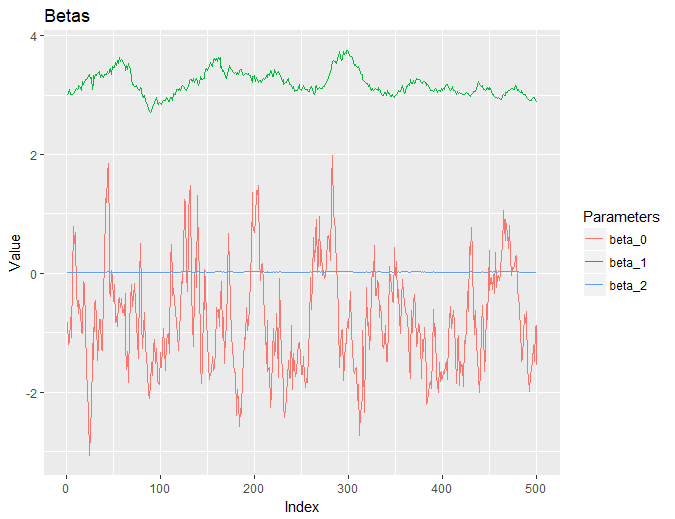
\includegraphics[width=\textwidth]{Chap3/GibbsChain}
        \caption{Trazas}
        \label{fig:GibbsChain}
    \end{subfigure}
	\quad
    \begin{subfigure}[b]{0.45\textwidth}
        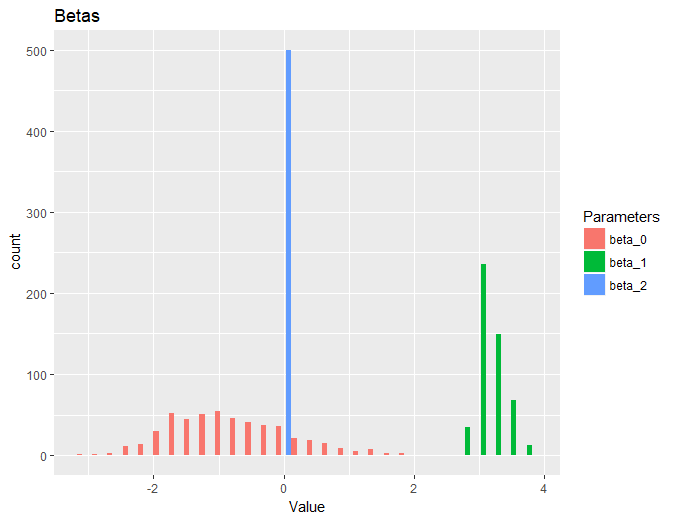
\includegraphics[width=\textwidth]{Chap3/GibbsHist}
        \caption{Histogramas}
        \label{fig:GibbsHist}
    \end{subfigure}
    \caption{Muestro Gibbs para el ejemplo \ref{ej:NormBiVar}}\label{fig:GibbsSamplerSimulado}
\end{figure}
Para esta figura, se toman los últimos 500 valores de las cadenas. Se observan las \textit{trazas} que se forman al ir simulando los parámetros y se hace un histograma, dando una idea de las distribuciones subyacentes\footnote{Estas imágenes tienen como propósito ejemplificar el Gibbs sampler. El modelo que se usa es el presentado en este trabajo. Asimismo, en el Capítulo \ref{cap:EjemYRes} se hará una exploración a fondo de este ejemplo en particular y se verá por que el parámetro $\beta_2$ es idénticamente cero, además de la razón por la que los histogramas se ven sospechosamente parecidos a una distribución normal. Asimismo, estas imágenes fueron generadas con la librería \textit{ggplot2}, incorporada a las funcionalidades del paquete \textit{bpwpm} desarrollado para este trabajo.}.\\

% Acabar parrafó con proceso de burnin y thinning. incluir comentario que esto lo hace el paquete. ;)
En la practica, muchos de los pormenores derivados del muestreo Gibbs, pueden ser mejorados. Dado que el valor inicial $\theta\iter{0}$ es dado por el estadista, en ocaciones el método tiene que explorar una región extensa de posibles valores para $\theta$, por lo que podría tardar en converger. Esto deriva en que las primeras observaciones deban ser descartadas pues no son realizaciones de la distribución final buscada. A este periodo se le conoce como \textit{burn-in}. En el ejemplo anterior, se utilizó $k^*$ para designar la iteración a partir de cual se toman los valores simulados. En la practica, usualmente se guarda toda la cadena, se explora, tanto por resúmenes numéricos como con representaciones gráficas y se decide (de forma subjetiva) el corte  $k^*$. Otro método ampliamente usado es el de adelgazamiento o \textit{thinning}. Por las mismas características de la estimación por Gibbs, sobre todo en casos multivariados, los valores de las cadenas tienen correlaciones altas. Si se quieren muestras independientes, la bibliografía recomienda tomar cada $\kthin$-ésimo valor de la cadena generada para reducir la dependencia entre los parámetros. Usualmente se usan valores pequeños para $\kthin$.  Estos sencillos pasos pasos para mejorar las cadenas, ya se encuentran implementados en el paquete \textit{bpwpm} para \verb|R| para el análisis rápido de las cadenas.

\subsection{Algoritmo de Albert y Chibb}
El algoritmo particular del Gibbs sampler que se usa en este trabajo, es una versión modificada del presentado en \autocite{albert1993bayesian}. Este método ofrece varias ventajas para esta aplicación en particular, pues se desarrolló específicamente para regresiones probit usando la variables latente $z$. Además es un método muy eficiente pues usa distribuciones conjugadas, por lo que las distribuciones condicionales, se puede calcular directamente y la parte estocástica depende únicamente de simular valores de una distribución normal multivariada. Esto lleva a que los periodos de burn-in sean relativamente pequeños y que el adelgazamiento no sea fundamentalmente necesarios.\\

A su algoritmo, ellos lo llaman \textit{Data Augmentation for Binary Data} y son los pioneros en el uso de variables latentes para unir la respuesta $y$ con las covariables $\xsn$ como se vió en la sección \ref{sec:GLM}. En su exposición, ellos no utilizan una función de proyección no lineal como la usada en este trabajo, sino, se restringen a la tradicional $f(\xsn) = \beta^t\xsn$. Por lo mismo (y por un breve momento) se utiliza la misma para explicar la idea fundamental. Usando la misma notación, se introducen $n$ variables latentes $\zsn = (z_1,\ldots,z_n)^t$, con $z_i \sim N(\beta^t\xni,1)$. Se definen las respuestas:
\begin{align}
y_i = 
	\begin{cases}
		1, & \text{si }\, z_i > 0 \\											0, & \text{si }\, z_i \leq 0 
	\end{cases} \label{ec:DefY}
\end{align}
La simplificación del modelo, obliga a que, por el momento $\theta = (\zsn, \beta)$. Por lo tanto, la derivación bayesiana es:
\begin{align}
	\pi(\zsn, \beta| \ysn, \xmat) \quad 
	& \alpha \quad \pi(\ysn | \xmat, \zsn, \beta) 
		\; \pi(\zsn, \beta) \nonumber \\
	& \alpha \quad \pi(\ysn | \zsn)\; \pi(\zsn|\beta,\xmat) 
		\; \pi(\beta) \nonumber \\
	& \alpha \quad \prod_{i = 1}^n[I(y_i = 1)I(z_i > 0) +
		 I(y_i = 0)I(z_i \leq 0)] \times \phi(z_i|\beta^t\xni,1) 				\times \pi(\beta) \label{ec:BayesChibbPosterior}
\end{align}

Ahora, bajo los fundamentos del Gibbs Sampler, en lugar de querer encontrar la distribución posterior (\ref{ec:BayesChibbPosterior}), se busca encontrar las distribuciones condicionales. Para $\beta$:
\begin{align}
	\pi(\beta|\zsn,\ysn,\xmat)
	& = \dfrac{\pi(\zsn, \beta| \ysn, \xmat)}{\pi(\zsn)} \label{ec:DefProbaCond}\\[5pt]
	& = \dfrac{\pi(\ysn | \zsn)\;\pi(\zsn|\beta,\xmat) 
	\; \pi(\beta)}{\pi(\ysn, \xmat) \; \pi(\zsn)} \nonumber \\[10pt]
	& = \cancelto{C}{\dfrac{\pi(\ysn | \zsn)}{\pi(\ysn, \xmat) \; \pi(\zsn)}} \times \pi(\zsn|\beta,\xmat) \; \pi(\beta) \label{ec:PasoDeLaMuerte} \\[5pt]
	& = C \,\pi(\beta) \, \prod_{i = 1}^n\phi(z_i|\beta^t\xni,1) \label{ec:BayesChibbBetaCond}
\end{align}
la densidad condicional completa es la misma que que la de una regresión lineal bayesiana donde $z_i = \beta^t\xni + e_i$ con $e_i \sim N(0,1)$. Es decir, al estar usando $z$ como regresor (dado) y condicionar sobre él, la simulación de $\beta$ se reduce a la que se haría sobre un modelo lineal bayesiano tradicional, asimismo, para estos modelos, dependiendo de $\pi(\beta)$ existen resultados cerrados. Se hace notar que la ecuación (\ref{ec:DefProbaCond}) se toma de la definición de probabilidad condicional, y el paso de (\ref{ec:PasoDeLaMuerte}) a (\ref{ec:BayesChibbBetaCond}) se puede hacer ya que, al definir $y$ como en la ecuación (\ref{ec:DefY}), sus representaciones son análogas y el cociente se desvanece, quedando únicamente la constante $C$ que sale del término $\pi(\ysn, \xmat)$. Ahora, únicamente falta definir $\pi(\beta)$. Es común en la práctica usar distribuciones \textit{no informativas} sobre los parámetros, cuando no se tiene experiencia sobre ellos. Sin embargo, para el modelo lineal bayesiano, existe una familia de distribuciones conjugadas \autocite{banerjee2008gory}. En particular, al dejar la varianza fija y eligiendo de distribución \textit{a priori} $\pi(\beta)$:
\begin{align}
	\beta \sim N_{d+1}(\beta|\mu_{\beta}, \Sigma_{\beta}) \label{ec:BetaAPriori}
\end{align}
donde $\mu_{\beta}\in \mathbb{R}^{d+1}$ es el hiperparámetro de media  y $\Sigma_{\beta} \in \mathbb{R}^{(d+1)^2}$ la matriz de covarianza,  entonces, se tiene la distribución conjugada:
\begin{align}
	\beta|\ysn,\zsn,\xmat &\sim N_{d+1}(\beta|\mu_\beta^*, \Sigma_\beta^*) 	\label{ec:SimBeta} \\
	\text{donde:}\quad& \nonumber \\
	 \mu_\beta^* &= \Sigma_\beta^* \times (\Sigma_\beta^{-1}\mu_\beta + \xmat^t\zsn )\nonumber \\
	 \Sigma_\beta^* &= (\Sigma_\beta^{-1} + \xmat^t\xmat)^{-1}\nonumber
\end{align}
Esta distribución es conjugada pues preserva la estructura normal de $\beta$. Asimismo, es fácil de simular usando cualquier software estadístico, calculando previamente todos los parámetros y dando un valor (o iteración) para $\zsn$\footnote{Se hace notar, que este estimador, es relativamente parecido al estimador que se da en una regresión cordillera.}.\\

Ahora, condicionar sobre $\zsn$, es más sencillo, pues la derivación es similar, comenzando con la expresión (\ref{ec:BayesChibbPosterior}) y reordenando términos:
\begin{align}
	\pi(\zsn|\beta,\ysn,\xmat)
	& = \dfrac{\pi(\zsn, \beta| \ysn, \xmat)}{\pi(\beta)} \nonumber \\[5pt]
	& = \dfrac{\pi(\ysn | \zsn)\;\pi(\zsn|\beta,\xmat) \; \pi(\beta)}			{\pi(\ysn, \xmat) \; \pi(\beta)} \nonumber \\[10pt]
	& = \cancelto{C}{\dfrac{1}{\pi(\ysn, \xmat)}}\pi(\ysn | \zsn) \times \pi(\zsn|\beta,\xmat) \nonumber \\[5pt]
	& = C \, \prod_{i = 1}^n[I(y_i = 1)I(z_i > 0) + I(y_i = 0)I(z_i \leq 0)] \times \phi(z_i|\beta^t\xni,1) \label{ec:BayesChibbZCond}
\end{align}
De donde es claro ver que las $z_i$ son independientes y tienen distribuciones normales truncadas en $0$:
\begin{align}
	z_i|y_i = 1,\beta &\sim N(z_i|\beta^t\xni,1) \text{ truncada a la izquierda} \label{ec:SimZ}\\
	z_i|y_i = 0,\beta &\sim N(z_i|\beta^t\xni,1) \text{ truncada a la derecha} \nonumber
\end{align}
las cuales también son fáciles de simular usando los algortimos de \autocite{devroye1986non}. \\

Finalmente, una vez que se tienen las distribuciones condicionales (\ref{ec:SimZ}) y (\ref{ec:SimBeta}), la simulación de esto dos primeros grupos de parámetros se realiza con un muestreo de Gibbs dado por las ecuaciones (\ref{ec:GibbsSampler}) de la página \pageref{ec:GibbsSampler}. En forma de pseudo-código:
\begin{verbatim} 
    SampleoGibbs(y, X, N_sim, beta(0), mu_beta, sigma_beta):
        sigma_beta <- Inv(Inv(sigma_beta) + X'X)
        PARA k = 1 HASTA N_sim:
            z(k) <- NormTrunc(y, X, beta(k-1))
            mu_beta(k) <- sigma_beta*(Inv(sigma_beta)*mu_beta + X'z(k))
            beta(k) <- NormMulti(sigma_beta(k)) 
        REGRESAR beta
\end{verbatim}
El valor de $\zsn\iter{0}$ en realidad no se tiene que dar; el valor inicial para $\beta\iter{0}$, puede ser dado por el estimador de máxima verosimilitud o el de mínimos cuadrados para las respuestas binarias $\beta\iter{0} = (\xmat^t\xmat)^{-1}\xmat^ty$. Sin embargo, en la práctica el algoritmo, por default, los inicializa en ceros y tardan poco tiempo en converger a la distribución límite. 

\subsubsection{Consideraciones adicionales para la simulación de $\wsn$}
% Poner las dos derivaciones de funciones condicionales (para las betas y para w)

%Argumentar por qué es igual para $w$ pero en lugar de usar las z de regresores se usan los residuales parciales.
%Mencionar que en el paper se hacen más algoritmos para diferentes cosas

%Distros a Priori
Para los parámetros, se usan las siguientes distribuciones \textit{apriori}:

\begin{align}
	\mathbf{\beta} &= (\beta_0,\beta_1,\ldots,\beta_d)^t \sim N_d(\mu_0, \Sigma_0) \\
	w\iter{i} &= (w\iter{i}_1,\ldots,w\iter{i}_J)^t \sim N_J(\mu\iter{i}_0,\Sigma\iter{i}_0) \quad i=1,\ldots,d
\end{align}

\section{Algoritmo \textit{bpwpm}}
En forma de pseudocódigo el algoritmo tiene la siguiente forma:

A diferencia de la exposición del modelo, el algoritmo debe de construir de abajo hacia arriba, pues se necesita tener una estimación puntual de los parámetros para poder calcular las funciones intermedias y que todo quede definido de forma numérica. 

% Mencionar el pedo de los cuantiles 

\begin{verbatim}
    Parametros inciales: 
    WHILE (...)
        Transformación de X -> Phi -> F (Función: estimate_PWP)		
        Simulación de betas (Función simulate_beta)
\end{verbatim} 

- Hacer énfasis en el apéndice y el paquete.

\subsection{Algoritmo de \textit{backfitting} para ajuste de modelos GAM} 
- Justificación final para las w's

% Te arrancas 
- Usamos los nodos iniciales en cuantiles determinados.\\
\begin{itemize}
\item taus: HMC
\item $\beta$ Estimar por máxima verosimilitud pero dentro del Gibbs con el método ABC
\item $w's$ BAyesianas + importantes que las betas.
\end{itemize}

- Explicar Alortimo y hacer pseudocódigo de cada sección
- Explicar lógica del algoritmo
- Explicar desarrolo de paquetes en R
- Explicar bien la parte de los residuales y el algorimto backfitting, por que las $f_j$ son arbitrarias y pueden interpolar a los residuales para hacer el ajuste. Esto también explica las $\beta$ pues si se pueden capturar chigón los residuales con una sola dimensión, te vale verga la siguiente :). Yei bitches

\begin{figure}[h]
\centering
\begin{tikzpicture}

% Dibujo nodos
\begin{scope}[
		every node/.style = {fill = white, shape = rectangle }]
		
	\node (t) at (-4,2) {$\t$};
	\node (Phi) at (-2,2) {$\Phi(x,\t)$};
	\node (w) at (-2,0) {$w_j\iter{k}$};
	\node (F) at (0,2) {$F\iter{k}$};
	\node (z) at (2,0) {$z\iter{k}$};	
	\node (beta) at (0,-2) {$\beta\iter{k}$};
	
\end{scope}

% Flechitas
\begin{scope}[
		every node/.style={fill = white, circle},
	    every edge/.style={draw = black, ->}]
	
	\path (t) edge  node [above] {cte.} (Phi);
	\path (Phi) edge (F);
	\path (F) edge [bend left](z);
	\path (z) edge [bend left](beta);
	\path (beta) edge [bend left](w);
	\path (w) edge[loop left] node [left] 
		{para $j = 1,\ldots,d \;$ }(w);
	\path (w) edge [bend left](F);

\end{scope}
\end{tikzpicture}
\caption{Esquema del algoritmo}
\label{fig:DiagramaAlgoritmo}
\end{figure}



\end{document}